\documentclass[sigsmall]{acmart}

\usepackage{graphicx}

\title{Summary of \emph{How Effective Are Commonly-Used Ad-Blockers?}}
\author{Matthew Oros, Sonny Smith, Michael Terekhov, Dennis Ulichney}

\setcopyright{none}
\settopmatter{printacmref=false}

\begin{document}
\maketitle


\section*{Abstract}
With the development of the internet web pages, online advertisements have also developed. Online advertisements can help find products that a user has been looking for, but they often ruin user experiences. Online advertisements might take up the whole space of a web page, and for mobile users, online advertisements might even make the usage of the page impossible. This research focuses on the software that removes such advertisements from web pages. The research paper includes an introduction, breakdown/related work, experiment design, results, and conclusion/future work.  

\section*{Introduction}
The services offered online are mostly free and the most common way to monetize them is through online advertising. Online ads can be helpful, but most users find them to be one of the most annoying things on the internet. Most internet users want to minimize the number of ads they see and various ad-blocking software can be used to achieve this. The easiest and most popular way to block ads is to use browser extensions. An advanced ad-blocking method is to use specialized software that blocks incoming ad domains. Advanced software is considered more reliable, which means it blocks more ads. The purpose of this study is to find out how effective ad-blocking extensions are. This study focuses on the most popular browser ad blockers and their effectiveness compared to Pi-Hole software (the advanced software used for this study). Ad-blocking extensions that were utilized are AdBlock Plus, AdBlock, uBlock Origin, Privacy Badger, and Ghostery. Internet browsers that were utilized to test the software are Chrome, Microsoft Edge, and Firefox.
[Man-in-the-Middle Proxy was also used to directly analyze the domains that were contacted when the extensions were active.]

\section*{Background/Related Work}
With the widespread use of ad-blockers, there have been numerous studies on their usage and effectiveness. One such study, for example, combined information from two million users from across the world with data on close to two trillion web requests to assess the usage and impact of ad-blockers across the Internet. The study found that, among other things, ad-blockers reduced the number of ads seen by about half, with the other half making it through \cite{10.1145/2987443.2987460}. Unlike our study, however, this one was more focused on the demographics of ad-blocker usage as well as some of its financial effects on website publishers. Because of this, it only looked at ad-blockers in a more general sense, instead of evaluating the performance of specific ones.

Another study, on the other hand, conducted a more specific analysis of the performance of different ad-blockers, many of which were also tested in our study. These ad-blockers were evaluated based both on how they affected the performance of the browser and how many user-tracking requests they blocked, with uBlock having the best performance. This study primarily differs from ours in its construction by looking at how ad-blockers affect browser performance, which we did not consider. Additionally, the study also only used one internet browser, Google Chrome, and also only made use of news websites, limiting the variety of the data collected \cite{10.1145/3091478.3091514}.

It is also worth mentioning that ad-blockers do not go unchallenged in their work, with an ongoing arms race between then[them] and advertisers. This, naturally, has resulted in a variety of methods for getting past ad-blockers. One such method, according to another study, is the use of replica ad domains. Replica ad domains are new advertising domains that advertisers will create in hopes of getting past the list of blocked domains that powers most ad-blockers. This method also seems to be highly effective at overcoming ad-blockers as well, with the researchers finding that some replica ad domains would, on average, extend the lifetime of both ads and trackers by 784.7 days before being blocked \cite{10.1145/3485447.3512218}. Furthermore, it is entirely possible, if not, likely that some of the advertisers on the websites looked at in our study have made use of this technique, which could have resulted in some ad domains flying under the radar of the ad-blockers that we used. Now, after looking at some of the past research on ad-blockers, we will detail our own methods and findings next.


\section*{Experiment Design}
Our testing methodology involves visiting a list of 30 websites with various ad-blocking extensions. We first recorded their effectiveness using the number of ads blocked reported by the extension. This information is self-reported by the ad-block[er] so we then compared the results of this data to our recorded results using a network proxy.

Ad-blocking extensions can work in various ways by[from] analyzing HTML elements on a webpage and comparing them to a known database to DNS to blocking DNS queries or a combination of multiple methods. Because of this flexibility, it can be difficult to fully assess the capabilities of a number of different ad-blocking extensions. In this study, we focused on the area of DNS query based blocking.

DNS stands for Domain Name System and is the system that maps human memorable domain names, such as google.com, to IP addresses that computers use to connect to a web server. DNS based blocking looks for requests the browser makes to certain domain names such as ads.google.com and instead of forwarding the request, blocks it by routing the domain to an invalid IP such as 0.0.0.0.

To test the effectiveness of the ad-blocker we use a proxy called MITM-Proxy to record all DNS (domain) requests when we visit each website. Using crowd-sourced ad-lists, we compared and counted how many of the domains requested are considered ads despite the ad-blocker being installed. This process was done using Python. Python was also used to create many of the visualizations used for our results.

Pi-hole is a DNS based ad-blocker and by using the same ad-lists that Pi-hole uses by default to test the effectiveness of the traditional ad-blocking extensions, we are able to predict the effectiveness of Pi-hole without having to actually run a Pi-hole instance. This allows us to compare the effectiveness of a DNS based ad-blocking solution to/with traditional ad-blocking extensions.

The outcome of the experiments include data about self-reported ads blocked by browsers extensions, number of ads per website tested, total requested domains per ad-blocker, and ratio of domains that are considered ads based on that total. The ratio is determined by which requested domains are also found in the default Pi-hole ad-list.
[If more filler is needed: name the ad-lists used and give some details about their origin]
\section*{Results}
The number of domains and ads blocked was first gathered from the blockers while in use and then gathered from proxy logs for comparison. The results of the first test found that uBlockOrigin detected and blocked the most domains on average followed by Ghostery and PrivacyBadger. uBlockOrigin blocked over 50\% more domains on average than the other blockers as shown in figure 1a. Although PrivacyBadger is not marketed as an adblocker, it blocked more domains on average than Adblock and Adblock Plus. 
AdBlock and AdBlock Plus blocked the lowest number of domains on average with mininal difference between the two blockers.  
 
The second test found that overall there were more domains and ads blocked by each blocker on average than reported by their icons as shown in figure 1b. Similarly to the first test, uBlockOrigin was found to block the most domains due to the fewest number of domains and ads being detected while it was active. With this test there was an inverse relationship with the blocker's performance and the number of domains detected and blocked. The fewer the amount of total domains and ads detected is, the better the blocker. uBlockOrigin had less than 200 total domains to block while the other blockers had more than 400 total domains which indicates that uBlockOrigin performed 50\% better than the other blockers in this test as well. Adblock Plus had the most total domains active of nearly 600. In comparison, Adblock, Ghostery, and PrivacyBadger all had around 450-475 total domains active. Adblock and Ghostery had similar total domain counts while Ghostery had a greater proportion of ad-domains. PrivacyBadger fell somewhere inbetwen Ghostery and Adblock in terms of total domain and ad-domain counts.   
\begin{figure}[h]
  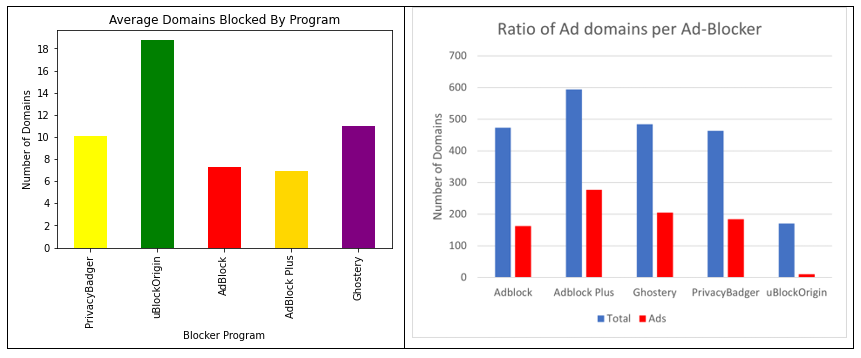
\includegraphics[scale = 0.75]{Edit3.png}
  \caption{ The leftmost graph(a) shows the average number of ad-domains reported by each adblocker. The rightmost graph(b) compares the total number of domains detected with a proxy to the number of those domains that are ads while each blocker was active.}
  \label{fig:graph1ab}
\end{figure}

\section*{Conclusion/Future Work}
In this study, we made use of the Stephen Black Hosts advertising domain list and a MITM Proxy server to compare the effectiveness of several popular ad-blocking extensions with Pi-Hole. These ad-blocking extensions consisted of AdBlock, AdBlock Plus, uBlock Origin, Ghostery, and Privacy Badger. To determine their effectiveness, we considered the number of domains that they claimed to block as well as the number of domains that still got through according to the MITM proxy. Using the Stephen Black Hosts list, the default filter list used by Pi-Hole, to identify ad domains that Pi-Hole would have blocked, we found that all of the ad-blockers tested blocked fewer ad domains from the list than Pi-Hole, with uBlock Origin blocking the most. Considering this, we conclude that using Pi-Hole will result in more ads being blocked than the ad-blocking extensions that we studied in this paper.

\bibliographystyle{acm}
\bibliography{myBib}
\end{document}
